\documentclass{beamer}

\usefonttheme{professionalfonts} % using non standard fonts for beamer
\usefonttheme{serif} % default family is serif

\usepackage{hyperref}
%\usepackage{minted}
\usepackage{animate}
\usepackage{graphicx}
\def\Put(#1,#2)#3{\leavevmode\makebox(0,0){\put(#1,#2){#3}}}
\usepackage{color}
\usepackage{tikz}
\usepackage{amssymb}
\usepackage{enumerate}


\newcommand\blfootnote[1]{%

  \begingroup

  \renewcommand\thefootnote{}\footnote{#1}%

  \addtocounter{footnote}{-1}%

  \endgroup

}

\makeatletter

%%%%%%%%%%%%%%%%%%%%%%%%%%%%%% Textclass specific LaTeX commands.

 % this default might be overridden by plain title style

 \newcommand\makebeamertitle{\frame{\maketitle}}%

 % (ERT) argument for the TOC

 \AtBeginDocument{%

   \let\origtableofcontents=\tableofcontents

   \def\tableofcontents{\@ifnextchar[{\origtableofcontents}{\gobbletableofcontents}}

   \def\gobbletableofcontents#1{\origtableofcontents}

 }

%%%%%%%%%%%%%%%%%%%%%%%%%%%%%% User specified LaTeX commands.

\usetheme{Malmoe}

% or ...

\useoutertheme{infolines}

\addtobeamertemplate{headline}{}{\vskip2pt}

\setbeamercovered{transparent}

% or whatever (possibly just delete it)

\makeatother

\begin{document}
\title[PFLOCK report]{PFLOCK Report}
\author[AC]{Andres Calderon}
\institute[Summer'19]{University of California, Riverside}
\makebeamertitle
\newif\iflattersubsect

\AtBeginSection[] {
    \begin{frame}<beamer>
    \frametitle{Outline} 
    \tableofcontents[currentsection]  
    \end{frame}
    \lattersubsectfalse
}

\AtBeginSubsection[] {
    \begin{frame}<beamer>
    \frametitle{Outline} 
    \tableofcontents[currentsubsection]  
    \end{frame}
}

\begin{frame}{LA\_10K Maximal disks finding (ICPE vs PFlock)}
    $\mu=3$.\\
    \centering
    \begin{figure}
        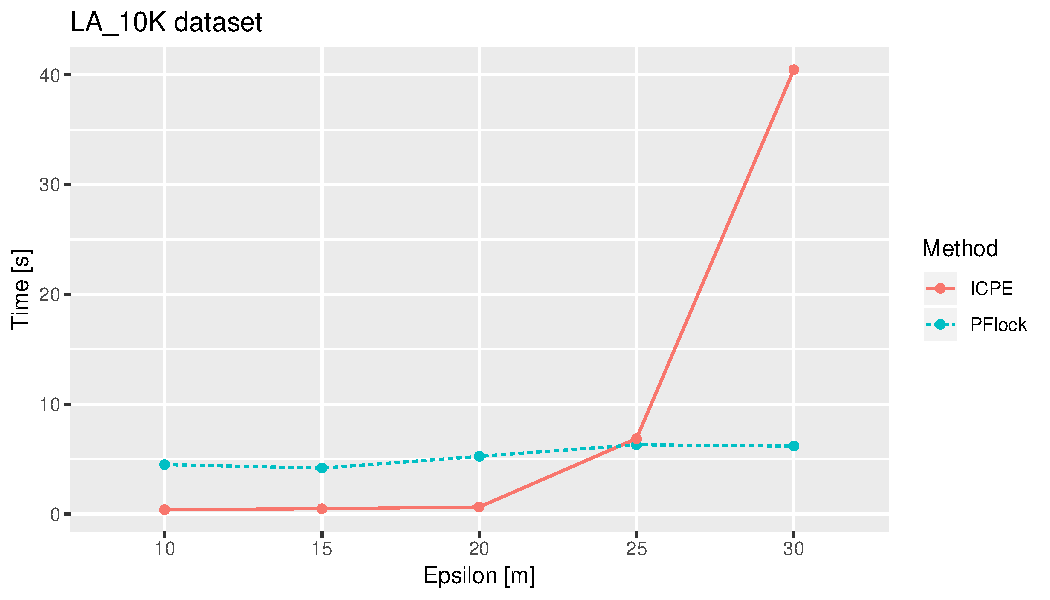
\includegraphics[width=\textwidth]{LA10K}
    \end{figure}    
\end{frame}

\begin{frame}{LA\_25K Maximal disks finding (ICPE vs PFlock)}
    $\mu=3$.\\
    \centering
    \begin{figure}
        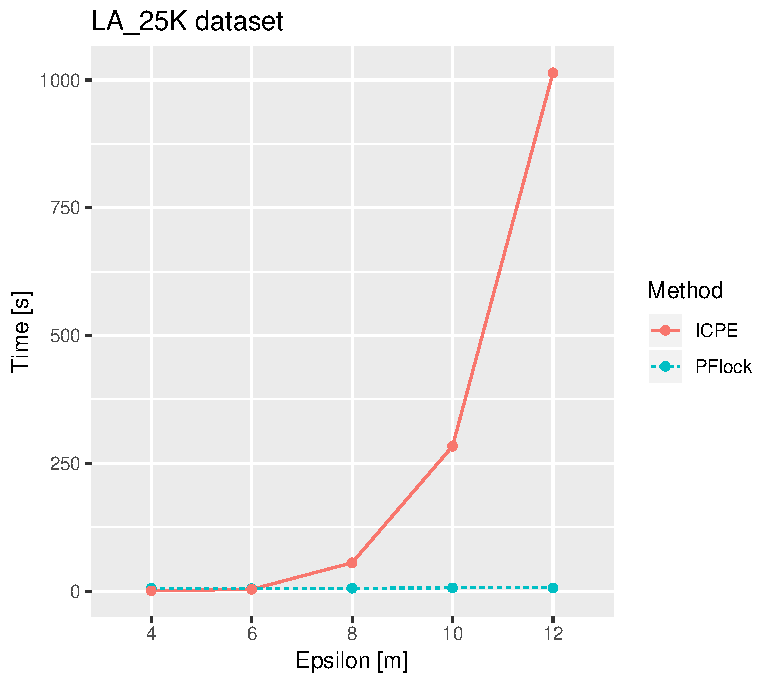
\includegraphics[width=\textwidth]{LA25K}
    \end{figure}    
\end{frame}

\begin{frame}{Some remarks (doubts)}
    \begin{itemize}
        \item ICPE proposes \textbf{Range Join}: The main purpose is to remove noise so DBScan would deal with only core and reachable points.  I perform this task throught a self distance-join using GeoSpark.  Is it a valid approach or I must follow the steps to built a Range Join?
        \item ICPE approach goes just until the cluster finding.  Up to this point, the approach is very fast.  The performance decrease after that, when it finds maximals disks following the BFE algorithm.
    \end{itemize}
\end{frame}

\begin{frame}{Some remarks (doubts)}
    \begin{itemize}
        \item ICPE claims it does not need to distribute the DBScan algorithm, so I neither distribute the BFE algorithm.  Both are sequential runnings.  It should be interesting to use the DBScan algorithm as a partitioner.
        \item Datasets from Chen et al. has duplicates and long jumps between their time instaces. The Brinkhoff dataset goes from 22M points to 9M after removing duplicates.
    \end{itemize}
\end{frame}

\end{document}
